This VR-application is in the context of a AR/VR-based surgical workflow as perviously described in Section \ref{chap::Approach}.
OMF surgeons can plan procedures with familiar surgical instruments on realistic representations of patients.
Workflows can be imported and exported via a file in JSON-notation.
The system uses a mixture of natural hand gestures like grabbing objects with voice commands for navigation.
The patient can be freely scaled, rotated and moved for visualization purposes.
Patients can be resetted to the default position on the operating desk at any time.

\begin{figure}[ht]
    \centering
    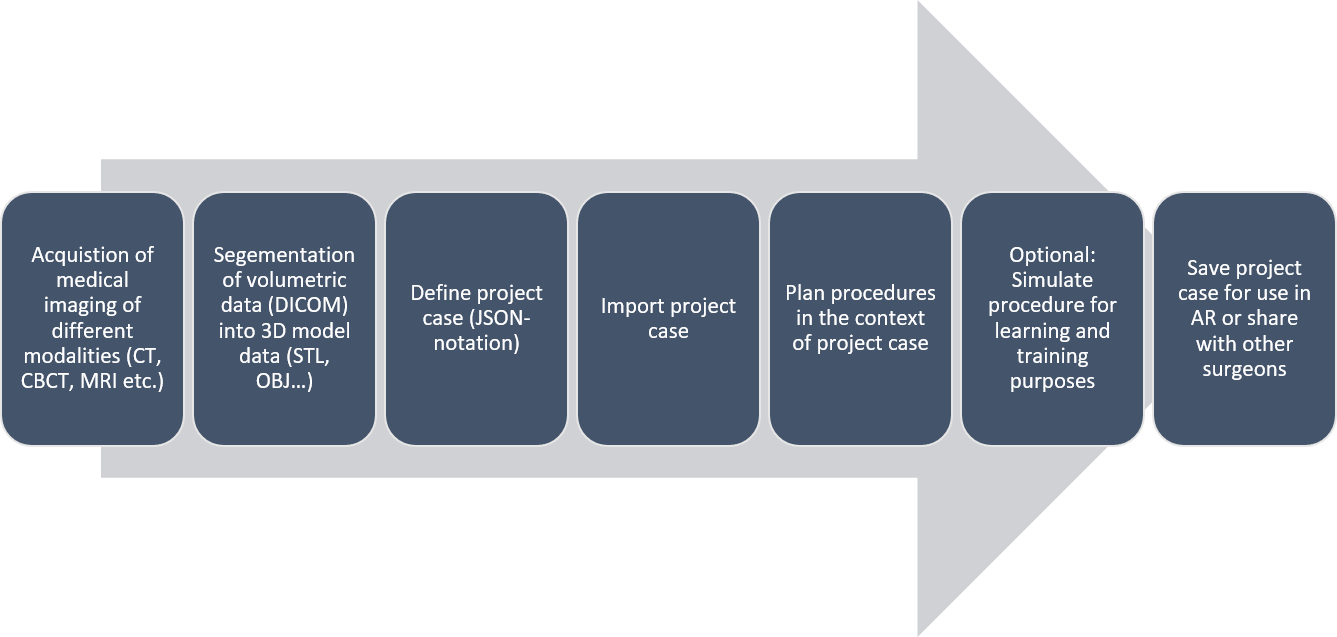
\includegraphics[width=350px]{images/implementation/workflow.png}
    \caption{\label{fig::ImplementationWorkflow}Step by step workflow of processing project cases in VR.}
\end{figure}

The workflow of the software is depicted in Figure \ref{fig::ImplementationWorkflow}.
Important to note is that the first two steps of the workflow are not part of this thesis, as they are provided in the scope of a different research project by the OMFS 
department of UHA.
The used 3D representations of surgical instruments, materials and the anatomical 3D models used for the development and evaluation of this thesis were prepared and provided in the scope of the aforementioned research project.
The anatomical 3D models are derived from BodyParts3D, The Database Center for Life Science licensed under CC Attribution-Share Alike 2.1 Japan \cite{mitsuhashi2009bodyparts3d}.
While segmenting the medical imaging in step two, the decision about which tissue has which color and which tissue will be transparant is made.
Specific features of the software are dependant on decisions made in these two steps.

The project case is at the core of the workflow since it acts as the interface between the independantly developed AR- and VR-software.
The specifics about the JSON-notation have already been agreed and decided upon in the conceptualization phase of the project, since it is critical for both of the applications to smoothly itneract. 

The case info contains patient specific information which is important for the procedure as depicted in the listing above.
These informations, aswell as the location of the patients 3d representation has to be manually registered by the user.
Information about the steps will be automatically generated while perfoming procedures inside of the application, however the user can then later add additional information as he sees fit.

The thought process behind this decision is that only medical experts themselves can know about the fine details while performing certain procedures.
Thus it is simply necessary to manually edit them with expert knowledge.
The automatically gernated information about the steps contains only information about which instrument was used at which step of the procedure.

When a project case is saved from within the application, a copy of the current patient with all steps which were performed is made withing the root folder of the patient model.
This way, the patients model is never lost and we can always start the procedure from scratch if desired.
Also, the timestamp of the updated field inside of the case info will be set.

When trying out the different apporaches as depicted in Setion \ref{sec::ConceptProjectCase}, we found that using this kind of approach is best suited for extensibility reasons.
By simply adding the planned procedures as additional 3D-Data to the patient, we ensure extensibility and robustness of the software.
New instruments and thus procedures can easily be added into the software without touching the project cases and everything will continue working as expected.
In comparison, if we used an approach where procedures have to be defined from within the project case, project cases would have to be updated every time we want to add new instruments to the application.

The tradeoff however, is that we can not adjust the procedures "on the fly" via text, but procedures have to be adjusted from within a 3D-modeling software or directly in the VR-application.
(TODO in implementation nichts hinterfragen, nur beschreiben)

After setting up the project case, it can be loaded up at runtime inside of the VR-application.
Users can then view, add and edit existing procedures or create new ones.
If users wish to run through the planned procedure step by step, they can either navigate through the procedure using the VUI or by enabling training mode, in which the user will 
be guided step by step through the procedure.
Here, users will be visually guided by the outlines of a surgical instrument to know where a procedure has to be performed.
Additionally, users will be guided via text inside of the application.
The text which is shown will be automatically generated with information about the current surgical instrument when performing a new procedure.
However, users are also free to edit the textual guidance manually via the JSON file in any way they see fit.
To confirm if the current procedure is carried out in the desired manner, voice feedback will notify the user if procedures are carried out correctly or if errors are being made.
The user can decide to save the current procedure for later use at any time of the process.